\chapter{Object Oriented Design}

\section{Robot}
Design a robot that will take your order and make sandwiches for you. 

Once I was done with this, I was supposed to extend it to have multiple robots doing this job like an assembly line handling multiple sandwiches and other edible items 

Once I handled that, he asked me to create a web service for this that will handle online ordering. He also wanted me to implement fulfillment centers

\subsection{分析}
1. Create Abstract class Item(it will have price and abstract prepare() method) \\
2. Create Sawdwich class,It will be extending Item class \\
3. Create Order class,It will have List<item> ,Customer Info \\
4. Robat as client,for accepting order,it will have list of orders,And will prepare items calling item's prepare method.

\section{sumBill}
Given an abstract class A having a function sumBill(int a, int b). Now assume that you have 3 or 4 class extending class A and implementing their version of sumBill. And in 
various locations in the code you are making calls to sumBill with integer parameters. 
Later on it is identified that the parameters need to be of type double rather than int. So now one has to go refactor all the places which make a call to sumBill to pass 
parameters of double data type. 
So the question is what could the developer had done better to avoid such a problem in the first place. 

\subsection{分析}
1. Method overloading:

Having an abstract overloaded method sumBill which accepts double parameter types and let derived classes override the method. It causes less flexibility to the developers as this 
technique will require the changes in every derived class. 

2. Encapsulation:

Box the primitive type integer or double in a user defined object and the object self sufficient to know the underlying the primitive data type. 

class A{ 
	sumBill(summableObject s1, summableObject s2); 
} 

3. Using Java.lang.Number class, you could pass any Integer, Double etc objects.. 
class A{ 
	sumBill(Number s1, Number s2); 
} 

\section{WebCrawler}
Design the algorithm and the system for a WebCrawler. 
The webcralwler will be provided millions of URLs. The webpage will be downloaded and then parsed for more URLs. If more URLs are found then they should also be downloaded and 
parsed. 

He was interested in: \\
1. Scale to handle millions of URLs \\
2. What are the bottle necks in the system? How will you resolve them

\subsection{分析}
Here is my design: \\
1, "Download worker". input: URL, output: URL \& documentation \\
2, "URL extract worker". Input: documentation, output: URLs \\
3, "URL feed". it accept URLs and then prepare to dispatch URLs to works. you can choose message queue or any technology. \\
4, "URL judgement". "URL extract worker" parse the document and output URLs. URL judgement component will lookup DB/memcache/... and decide if we need add all or parts fo URLs to 
"URL feed". \\
5, URL key and value storage. the value can includes URL expiration time, URL downloaded document location, size, ... we can use memcache, DB... \\
6, background thread. it can check the URL key and value storage periodically. if a URL expired, we send the URL to "URL feeder" to update the documents and URLs 

\section{Vending Machine}
Design a vending machine

\subsection{分析}
class Item < describes the various items in the vending machine> 

class ProductCode < to select which drink/snack you want> 

class Coin < to accept coins> 

class Refund < to return remainder coins> 

class Stock < to keep track of the vending machine stock for each product> 

class Bagel, Donut, Energy bar, Chocolates extends class Item

\section{Parking System}
Design a valet parking system. Requirements of the valet parking system should be: \\
1. Customer are given a ticket that they can use to redeem to get their vehicle back \\
2. Parking spots come in three sizes, small, med, large \\
3. Thee types of vehicles, small, med, large \\
-a small vehicle can park in a small, medium, and large spot \\
-a medium vehicle can park in a medium and large spot \\
-a large vehicle can park in a large spot\\

\subsection{分析}
\begin{Code}
	class Ticket {
		public string PersonName;
		public string TicketID;
	}
	
	class ValetParking{
		private Dictionary<Ticket, Spot> ticketRemainder = new Dictionary<Ticket, Spot>();
		private List<Spot> smallSpots = new List<Spot>();
		private List<Spot> mediumSpots = new List<Spot>();
		private List<Spot> bigSpots = new List<Spot>();
		
		public ValetParking(int small, int medium, int big) {
			CreateSpots(small, VehicleSize.Small);
			CreateSpots(medium, VehicleSize.Medium);
			CreateSpots(big, VehicleSize.Big);
		}
		
		private void CreateSpots(int total, VehicleSize type) {
			List<Spot> list = null;
			switch (type) {
				case VehicleSize.Small:{
					list = smallSpots; break;
				}
				case VehicleSize.Medium:{
					list = mediumSpots; break;
				}
				case VehicleSize.Big:{
					list = bigSpots; break;
				}
			}
			
			for (int i = 0; i < total; i++){
				list.Add(new Spot(type));
			}
		}
		
		private Spot FindSpot(Vehicle v) {
			if (v == null) return null;
			
			List<List<Spot>> spotsToSearch = new List<List<Spot>>();
			
			spotsToSearch.Add(smallSpots);
			
			if (v.Size == VehicleSize.Medium || v.Size == VehicleSize.Big) {
				spotsToSearch.Add(mediumSpots);
			}
			if (v.Size == VehicleSize.Big){
				spotsToSearch.Add(bigSpots);
			}
			
			foreach (List<Spot> parking in spotsToSearch) {
				foreach (Spot s in parking){
					if (!s.IsEmpty) {
						return s;
					}
				}
			}
			
			return null;
		}
		
		public Ticket Park(Vehicle v, string personName) {
			
			Spot s = FindSpot(v);
			
			if (s != null) {
				s.Park(v);
				Ticket t = new Ticket() { PersonName = personName, TicketID = "Ticket ID : " + s.GetHashCode() };
				ticketRemainder.Add(t, s);	
				return t;
			}
			return null;
		} 
		
		public Vehicle Unpark(Ticket ticket) {
			if (ticket != null && ticketRemainder.ContainsKey(ticket)) {
				Spot s = ticketRemainder[ticket];
				return s.Unpark();
			}
			return null;
		}
	}
	
	public enum VehicleSize { Small, Medium, Big }

	class Vehicle {
		private VehicleSize size = VehicleSize.Small;
		public VehicleSize Size {
			get { return size; }
		}
	}
	
	class Spot {
		private VehicleSize size = VehicleSize.Small;
		public VehicleSize Size{
			get { return size; }
		}
		
		public Spot(VehicleSize vs) {
			size = vs;
		}
		
		private Vehicle ParkedVehicle { get; set; }
		
		public void Park(Vehicle v) {
			if (IsEmpty){
				ParkedVehicle = v;
			}
		}
		
		public Vehicle Unpark() {
			if (!IsEmpty) {
				Vehicle v = ParkedVehicle;
				ParkedVehicle = null;
				return v;
			}
			return null;
		}
		
		public bool IsEmpty {
			get { return ParkedVehicle == null; }
		}
	}
\end{Code}

\section{Operator}
Implement << operator. What are the differences of implementation as a member function and a non-member function

\section{Like Functionality}
Design a system like friend's functionality in facebook. should have all features of facebook's friends functionality. like for each person , he can have any number of friends , 
he will get suggestions for new firends , showing common friends if we visits any other profile . algo should be scalable , robust .

\subsection{分析}
Basically a friends network is an undirected graph. Each person is a vertex of the graph and friendship is an edge between the two vertices. We can represent the graph by by 
maintaining an adjacency list. \\
- Like: Each person maintains a list of Posts. Lets say person A puts a post, persons who are connected to person A will be notified about the post (observer pattern). Friend B 
can like a post which increase the 'Like' count. \\
- Friends Suggestion: For person A find all nodes X that is at distance 2 from node A. (Now this is scalable as the requirements can tell what is the depth we want to look for 
making suggestions.) \\
- Common Friends: When A visits person B. Find all nodes X that are at distance 1 from node A.

\section{Casino}
To design classes and methods for casino cards games, what would you consider when doing it?

\subsection{分析}
\begin{Code}
	//Suit: 
	//	Club = 0 
	//	Diamond = 1 
	//	Heart = 2 
	//	Spade = 3 
	//
	//Color: 
	//	Black = 0 
	//	Red = 1
	//	
	class Cards {
		private:
		int m_suit ;
		int m_rank ;
		
		public:
		Cards ( int r, int s ) {
			m_rank = r ;
			m_suit = s ;
		}
		
		int getRank ( ) { 
			return m_rank ;
		}
		
		int getSuit() {
			return m_suit ;
		}
		
		int getColor ( int suit ) {
			return ((1 == suit) || (2 == suit))? 1 : 0 ;
		}
		
		string toString (int rank) {
			string val ;
			switch (rank) {
				case 1 :
				val = "Ace" ;
				break ;
				.....
				.....
				case 10:
				val = "Jack" ;
				break ;
				case 11:
				val = "Queen" ;
				break ;
				case 12:
				val = "King" ;
				break ;
				default:
				break ;
			}
			return val ;
		}
	}
	
	class CardDeck{
		private:
		Card[] m_deck ;
		int m_numCards ;
		public:
		CardDeck() {
			m_deck = new Card[52] ;
			initCards() ;
		}
		
		void initCards() {
			int idx = 0 ;
			for ( int rank = 1; rank <= 13; rank++ ) {
				for ( int suit = 0; suit < 4; suit++ ) {
					m_deck[index] = new Card(rank,suit) ;
					index++ ;
				}
			}
			m_numCards = 52 ;
		}
		
		int getSizeOfDeck () {
			return m_numCards ;
		}
		
		Card deal () {
			if ( 0 == m_numCards )
			return NULL;
			m_numCards-- ;
			return m_deck[m_numCards] ;
		}
		
		void shuffle() {
			for ( int next = 0; next < m_numCards-1; next++ ) {
				int rdm = myRandom(i, m_numCards-1) ;
				Card temp = m_deck[next] ;
				m_deck[next] = m_deck[rdm] ;
				m_deck[rdm] = temp ;
			}
		}
		
		static int myRandom ( int low, int high ) {
			return (int) ( (high+1-low) * Math.random() + low ) ;
		}
	}
\end{Code}

\section{Logger}
Design a logger class for your application? The log messages can be printed in a log file. 
Suppose you may want to provide the user the option whether he wants to print the messages in a log file or into database at runtime. How would you modify your earlier design?

\subsection{分析}
\begin{Code}
	class Logger {
		private:
		bool db_flag;
		string log_name;
		static Logger *m_pInstance; 
		Logger (){};
		Logger(const Logger &);
		Logger &( operator =(const Logger &) {};
		
		
		public:
		static Logger * Instance() {};
		bool openlogfile(bool flag,string logname);
		void writetoLog();      
		bool closeLog();
		
	}
	
	Logger * Logger::m_pInstance = NULL;
	Logger * Logger :: Instance(bool flag,string logname) {
		if (!m_pInstance) 
		m_pInstance = new Logger(flag,logname);
		
		return m_pInstance;
	}
	
	bool Logger::openlogfile(bool flag,string logname) {
		db_flag = flag;
		log_name = logname;
		if (db_flag){
			//connect to DB
		} else
		open (logname);
	}
\end{Code}

\section{Tree Serialize and Deserialize}
Given a tree - not necessarily a binary tree - the serialize method should create a string for the tree. The deserialize method should be able to reproduce the same tree using the 
string derived from the serialize method. 

Basically, serialize() takes in a tree and returns a string, deserialize() takes in a string and returns the tree.

\subsection{分析}
\begin{Code}
	class Node {
	public:
		Data d;
		list<Node*> children;
		
		void Serialize() {
			// write my data
			cout << d;
			
			// write the number of children
			cout << children.size();
			
			// write my children
			for(auto itr=children.begin(); itr != children.end(); ++itr) itr->serialize();
		}
		
		void deserialize() {
			// read my data
			cin >> d;
			
			// read my number of children
			int num_children;
			cin >> num_children;
			
			// read the children
			while(num_children-- > 0) {
				Node* pNode = new Node();
				pNode->deserialize();
				children->push_back(pNode);
			}
		}
	};
\end{Code}

\section{Furniture}
A furniture can be made of material like metal, wood, .... Also there are different furniture types chair, table, sofa. A wood furniture should be tested against choaking. metal 
furniture is tested against fire, etc. Design these in OOAD.

\subsection{分析}
\begin{Code}
	enum FurnitureType {
		WOOD, METAL;
	}
	
	abstract class Furniture {
		FurnitureType furnitureType;
		FurnitureTest furnitureTest;
		
		public Furniture(FurnitureType furnitureType, FurnitureTest furnitureTest) {
			this.furnitureType = furnitureType;
			this.furnitureTest = furnitureTest;
		}
		
		public boolean testFurniture() {
			return furnitureTest.testFurniture();
		}
		
	}
	
	interface FurnitureTest {
		public boolean testFurniture();
	}
	
	class WoodFurnitureTest implements FurnitureTest {
		public boolean testFurniture() {
			/*
			* Test code goes here
			*/
			return true;
		}
	}
	
	class MetalFurnitureTest implements FurnitureTest {
		public boolean testFurniture() {
			/*
			* Test code goes here
			*/
			return true;
		}
	}
	
	class Chair extends Furniture {
		public Chair(FurnitureType furnitureType, FurnitureTest furnitureTest) {
			super(furnitureType, furnitureTest);
		}
	}
	
	class Table extends Furniture {
		public Table(FurnitureType furnitureType, FurnitureTest furnitureTest) {
			super(furnitureType, furnitureTest);
		}
	}
	
	class TestClient {
		public static void main(String[] args) {
			
			WoodFurnitureTest woodFurnitureTest = new WoodFurnitureTest();
			MetalFurnitureTest metalFurnitureTest = new MetalFurnitureTest();
			
			// create wood chair
			Chair woodchaChair = new Chair(FurnitureType.WOOD, woodFurnitureTest);
			
			// create metal chair
			Chair metalChair = new Chair(FurnitureType.METAL, metalFurnitureTest);
		}
	}
\end{Code}

\section{Pool}
Design a Pool class and write down any interfaces that you could think? A Pool class could be a Thread Pool or memory pool, that can store resources.

\subsection{分析}
This is a contextual question and is specially based on the architecture of the component or the product you are using. However, assuming the general structure, I would classify 
as follows. 

Class Pool having members as \\
1> Number_of_resources. \\
2> Thread_count / memory_constraints. \\
3> semaphore_variable // to lock \& unlock No_of_resources . \\
etc. 

Now for that interface would be like. 

1> getSystemthread() // which will give a new thread if possible. \\
2> releaseThread(threadID ). 


This question goes on with the discussion panel as the question have a vast scope. like Singleton design Pattern should control the thread access and mechanism to overcome 
deadlock using semaphore has to be designed with.

\section{C++ Class}
What are general guidelines you follow while creating new classes in C++ 

\subsection{分析}
My answer: \\
1. Keep variables pvt (use setter and getter methods) \\
2. Use reference counting to do mem management, he asked me to use shared_ptr within the class\\

My understanding is as following apart from the above answers. Please correct me if you think something is not feasible. \\
1. We need to think whether we want to create an abstract class (making some of its method as pure virtual). If there is a possibility of extending the behaviors of this class we 
can make some of its member function as virtual. \\
2. On the other hand, if the class has to used with different data types and there is not much change in the behavior (i.e. member functions) for data types, we can create a 
template class. For example while writing any container class we may think of making it a template class, so that different data types can be stored inside the container class. 
This would depend upon the business use case for which we are designing/writing the class.

1. What's the class used for? You cannot include everything or too much in one class. \\
2. You are going to create an abstract class or a class inheriting another? \\
3. Namespace, Constructors, Members, Properties, Methods, etc. \\
4. The role of this class in your design/architecture/model. 

1.private variables. \\
2.public get and set methods  \\
3.multiple constructor-without args,with 1,2,3,... args,copy constructor \\
4.do i need to overload operators? +,-,=. eg.in matrix class overloading + will simplify usage \\
5.destructor. free memory if you allocated any \\
6.Do I need virtual functions or an abstract class or just a simple class?

\section{Game}
It has different types of monsters and different weapons. hero would shoot monster. each monster would have some initial health. Each weapon would do some predefined damage to 
monster. when its health gets 0, monster would die/disappear. and there would be multiple levels. based on level, monster and their behavior would change.

\subsection{分析}
\begin{Code}
	public class Weapon{ 
		String name;
		int damagingEffect; 
		int bulletsLeft;
		
		public Weapon(name, damagingEffect, bulletsLeft) {// initialize all}
		
		// returns damaging effect
		public int fireWeapon() {
			if (bulletsLeft == 0) {
				throw new OutOfAmmoException(name);
			}
			bulletsLeft--;
			return damagingEffect;
		}
		
		public void reload(int newBullets) {
			bullets+= newBullets;
		}
	}
	
	public class Hero {
		Map<String, Weapon> weapons = new HashMap<String, Weapon>();
		Weapon currentWeapon;
		
		public Hero(Set<Weapon> weapons) {
			for(Weapon weapon:weapons) 
			this.weapons.put(weapon.name(), weapon);
			currentWeapon = weapons.get(0);
		}       
		
		public void setCurrentWeapon(String name) {
			if (!weapons.contains(name)) {
				throw new NoSuchWeaponException(name);
			}
			currentWeapon = weapons.get(name);
		}
		
		// returns damaging effect
		public int fire() {
			return currentWeapon.fireWeapon();
		}
		
		public boolean isUnArmed() {
			// check and return true if all weapons are out of bullets
		}
	}
	
	public class Monster {
		String name;
		int health;
		
		public Monster(String name, int health) {// initialize}
		
		// returns true if dead
		public boolean damageHealth(int damageEffect) {
			health-=damageEffect;
			return isDead();
		}
		
		public boolean isDead() { 
			return health<=0;
		} 
	}
	
	public class Game {
		Hero hero;
		int level;
		Map<String, Monster> monsters;
		enum LevelResult {WON, LOST, PLAYING};
		
		public Game(Hero hero, Set<Monster> monsters, int level) {//initialize}
		
		public void doEncounter(String monsterName) {
			Monster monster = monsters.get(monsterName);
			boolean isDead = monster.damageHealth(hero.fire());
			if (monster.isDead()) {
				monsters.remove(monsterName);
			}
		} 
		
		public void misFire() {
			hero.fire(); // didn't hit any monster
		}
		
		public LevelResult getLevelResult() {
			if (mosters.isEmpty()) { 
				return LevelResult.WON;
			} else if (hero.isUnArmed()) {
			return LevelResult.LOST;
			} else {
				return LevelResult.PLAYiNG;
			}
		}
	}
\end{Code}

\section{Elevator}
How to design an elevator system. Main thing to worry about is how would you notify the elevator that it needs to move up or down. and also if you are going to have a centralized 
class to control this behavior and how could you distribute the control.

\subsection{分析}
\begin{Code}
	public class Elevator {
		
		public static final int MAX_FLOORS = 50;
		
		// upward floor queue
		private PriorityQueue<Integer> floors_up = new PriorityQueue<Integer>(MAX_FLOORS);
		
		// downward floor queue
		private PriorityQueue<Integer> floors_down = new PriorityQueue<Integer>(MAX_FLOORS, new Comparator<Integer>(){
			public int compare(Integer arg0, Integer arg1) {
				return arg1.compareTo(arg0);
			}
		});
		
		// effective floor queue
		private PriorityQueue<Integer> floors = floors_up;
		
		// current floor
		private int current = 0;
		
		public void userCallAt(int where) {
			setTarget(where);
		}
		
		public void setTarget(int target) {
			
			// ignore if target is current
			if (target == current) {
				return;
			}
			
			// add target to right queue
			if (floors == floors_up) {
				if (target < current) {
					floors_down.offer(target);
				} else {
					floors_up.offer(target);
				}
			} else {
				if (target > current) {
					floors_up.offer(target);
				} else {
					floors_down.offer(target);
				}
			}

			// swap queue to turn around the elevator
			if (floors.isEmpty()) {
				floors = (floors == floors_up ? floors_down : floors_up);
			}
		}

		public int getTarget() {
	
			if (!floors.isEmpty()) {
				return floors.peek();
			}
	
			if (floors_up.isEmpty() && floors_down.isEmpty()) {
				return current;
			}
	
			floors = (floors == floors_up ? floors_down : floors_up);
			return floors.peek();
		}

		public int getCurrent() {
			return current;
		}

		public void step(int target) {
			if (target > current) {
				current++;
			} else {
				current--;
			}
		}

		public void stop() {
			floors.poll();
		}

		public void move() {
	
			while (getCurrent() != getTarget()) {
				do {
					step(getTarget());
				} while (getCurrent() != getTarget());
				stop();
			}
		}
	}
\end{Code}

\section{Mutiple Elevator}
Design a multiple elevators system of skyscraper. Design an algorithm to let person find available elevator soon. How to improve your algorithm?

\begin{Code}
	class ElevatorManager{
		Elevator elevatorArray[ELEVATOR_COUNT];
		// List of pending hallcalls
		HallCallList hallcallList_;
		
		public:
		// User API to intiate a hall call
		void ProcessHallCall(const HallCall& rHallCall);
		
		private:
		// Starts the Hall Call Process Thread
		void StartHallCallProcessThread();
		// Create thread for each elevator to make it operational
		void StartCarMovementThread();
	};
	
	void ElevatorManager::ProcessHallCall(const HallCall& rHallCall){
		hallcallList_->AddHallCall(rHallCall);
	}
	
	ElevatorManager::StartHallCallProcessThread(){
		HallCallProcessThread thread(elevator, hallcallList_);
		thread.run();
		thread.detach();
	}
	
	ElevatorManager::StartCarMovementThread(){
		for (int i = 0; i < ELEVATOR_COUNT; i++){
			ElevatorThread thread(elevatorArray[i]);
			thread.run();
			thread.execute();
		}
	}
	
	
	//////////////////////////////////////////////////////////////////////////////////
	
	// class encapsulating the hallcall list treatment
	class HallCallList{
		list<HallCall> lHallCallList_;
		Mutex mHallCallListMutex;
		public:
		void AddHallCall(HallCall hallCall);
		HallCall PopHallCall();
	};
	
	HallCallList::AddHallCall(HallCall hallCall){
		MutexLock(mHallCallListMutex);
		lHallCallList_->push_back(hallCall);
		hallCallListSemaphore->signal();
	}
	
	HallCall HallCallList::PopHallCall(){
		MutexLock(mHallCallListMutex);
		Hallcall hallcall = lHallCallList_->front();
		lHallCallList_->erase(lHallCallList_.begin(), lHallCallList_.begin());
		return hallcall;
	}
	
	//////////////////////////////////////////////////////////////////////////////////
	// Creates one thread per hallcall so that non-interfering hall calls can work parallely
	HallCallProcessThread::Execute(){
		hallCallListSemaphore->signal();
		MutexLock(mHallCallListMutex);
		Hallcall hallcall = hallcallList_->pop();
		OneHallcallThread thread(hallcall, hallcallList_);
		thread.run()
		thread.detach();
	}
	
	OneHallcallThread::Execute(){
		bool bCallProcessed = false;
		// Sorted Elevator Array sorts the provided elevator array based on the current requested hallcall floor.
		// We want to try out the elevator which is nearest
		SortedElevator elevatorArray(elevatorArray, hallcall);
		FOR_EACH elevator in elevatorArray{
			if (true == elevator->ProcessCall(hallcall)){
				bCallProcessed = true;
				break;
			}
		}
		
		// If currently no elevator can process the hallcall
		// it is added back to the hallcalllist
		if (false == bCallProcessed){
			hallcallList_->AddHallCall(hallcall);
		}
	}
	
	
	/////////////////////////////////////////////////////////////////////////////////////////////
	
	class Elevator{
		typedef int FLOOR;
		typedef list<FLOOR> DestFloorList;
		Mutex elevLock;
		Semaphore destFloorEmptySem; // To put elevator thread into wait state when no hallcall
		DestFloorList lDestFloorList_;
		public:
		Elevator() : elevLock(1), destFloorEmptySem(0);
		void ProcessCall(Hallcall hallcall);
		void Move();
		
		protected:
		void Reset();
		void UpdateCurrentFloor();
	};
	
	Elevator::ProcessCall(HallCall hallcall){
		Mutexlock lock(elevLock);
		
		// Logic to find if the elevator can process the request
		if ((this->state == STATIONARY) || 
		((this->state == UP) && (hallcall.direction == UP) && (this->currFloor < hallcall.floor)) ||
		((this->state == DOWN) && (hallcall.direction == DOWN) && (this->currFloor > hallcall.floor))){
			this->lDestFloorList_->push_back(hallcall.floor);
			this->destFloorEmptySem_->signal();
			return true;
		}
		
		return false;
	}
	
	Elevator::Reset(){
		this->state = STATIONARY;
		this->currFloor = 0;
		this->lDestFloorList_ = empty List;
	}
	
	Elevator::UpdateCurrentFloor(){
		Mutexlock lock(this->elevLock);
		Floor targetFloor = this->lDestFloorList_->front();
		if (this->currFloor > targetFloor){
			this->state = DOWN;
			this->currFloor--;
		}
		else if (this->currFloor < nextFloor)	{
			this->state = UP;
			this->currFloor++;
		}
	}
	
	ElevatorThread::Execute(){
		elevator->Move();
	}
	
	Elevator::Move(){
		this->Reset();
		while(true) {
			if ((this->state == UP) ||  (this->state == DOWN)){
				floor = this->lDestFloorList_->top();
				if (floor == this->currFloor){
					{
						Mutexlock lock(elevLock);
						this->lDestFloorList_->pop_front();
						this->state == STATIONARY;
					}
					this->destFloorEmptySem_->wait();
					this->UpdateCurrentFloor();
				}
				else{
					this->UpdateCurrentFloor();
				}
			}
			else{
				this->destFloorEmptySem_->wait();
				this->UpdateCurrentFloor();
			}
			sleep(5);
		}
	}
\end{Code}

\section{Coffee Shop}
Design Coffee Shop? Follow up: Extend this to handle multiple coffee shops (Ex like starbucks and across countries)

\subsection{分析}
\begin{Code}
	typedef long ID;
	
	enum Roll {CASHIER, MANAGER, WAITER};
	class Employee{
		ID empID;
		string name;
		Roll roll;
		public:
		setRoll ();
	}
	
	class Waiter: public Employee{
	public:
		waiter() {	setRoll (WAITOR); }
	}
	
	class Cashier: public Employee{
	public:
		cashier () {	setRoll (CASHIER); }
	}
	
	class Table{
		ID tableId;
		bool isAvailable;
		int capacity;
		int used;
		
	public:
		Table(ID id) {tableId = id; // set other params also}
		
		bool isAvailable ();
		void reserveTable ();
		void freeTable ();
	}
	
	Class Item{
		ID itemID;
		double itemCost;
		public:
		getItemCost ();
	}
	
	class Order{
		Table tableID;
		Waiter waiterID;
		Cashier cashierID;
		
		vector<item, int> request; // item, quantity
		public:
		void placeOrder (itemID, quantity) ;// push_back in request vector
		double getBill (); // call Invoice Class's generateBill()
	}
	
	class Menu{
		map<item, double> itemCostMap; //
		map<item, int> itermQuantityMap; //
		
	public:
		double getItemCost (Item itemID);
		int getItemQuantity (Item itemID);
		bool isItemAvailable (Item itemID);
	}
	
	class invoice{
		Menu menu;
	public:
		generateBill (vector<itemID, quantity>); // uses Menu class getItemCost () to get cost and generate bill
	}
	
	
	class coffeeShop{
		List<Table> tables;
		List<Waiter> waiters;
		List<Cashier> cashiers;
		map<Table, Order> orders;
		
	public:
		coffeeShop (){
			//initialise each table with ID and capacity; and other member also;
		}
		void addWaiter ();
		void removeWaiter ();
		void addCashier();
		void removeCashier ();
		//similar for other employees, like manager 
		
		void addTable ();
		void removeTable():
		
		void getOrder (Table tableId, Item itemID, int quantity); // this will order object and place in map
		
		double getBill (Table tableId){ 
			Order order = orders[tableId]; 
			order.getBill ();
		}
	}
\end{Code}

\section{Card}
Design a class for Game of card. You can use any design pattern or data structure. \\
1. There are 52 card. \\
2. There are 4 suits, each contain 13 cards.

\subsection{fen'xi分析}
\begin{Code}
	#include <iostream> 
	#include <algorithm>
	#include <vector>
	
	using namespace std; 
	
	enum CardSuite{
		CARD_CLUB, 
		CARD_HEART,
		CARD_SPADE, 
		CARD_DIAMOND
	};
	
	enum CardNumber {
		CARD_ONE = 1,
		CARD_TWO,
		CARD_THREE,
		CARD_FOUR,
		CARD_FIVE,
		CARD_SIX,
		CARD_SEVEN,
		CARD_EIGHT, 
		CARD_NINE,
		CARD_TEN,
		CARD_JACK,
		CARD_QUEEN,
		CARD_KING	
	};
	
	class OneCard{
		CardSuite eSuite_;
		CardNumber eNumber_;
	public : 
		OneCard(CardSuite suite, CardNumber num){
			eSuite_ = suite;
			eNumber_=num;
		}
		CardSuite GetSuite(){
			return eSuite_;
		}
		CardNumber GetNumber() {
			return eNumber_;
		}
		void Decompile(){
			cout << eSuite_ << " " << eNumber_ << endl;
		}
	};
	
	class CardDeck{
		vector <OneCard> cardDecks_; 
		public:
		CardDeck(){
			CardSuite suite;
			CardNumber cNumber;
			for (suite = CARD_CLUB; suite != CARD_DIAMOND + 1; suite = static_cast<CardSuite>(suite + 1)){
				for (cNumber = CARD_ONE; cNumber != CARD_KING + 1; cNumber = static_cast<CardNumber>(cNumber + 1)){
					OneCard card = OneCard(suite, cNumber);
					cardDecks_.push_back(card);
				}
			}
		}
		
		void RandomizeCards(){
			std::random_shuffle(cardDecks_.begin(), cardDecks_.end());
		}
		
		void Decompile() {
			vector<OneCard> :: iterator iter = cardDecks_.begin();
			while (iter != cardDecks_.end()){
				(*iter).Decompile();
				iter++;
			}
		}
	};
	
	
	int main( ){ 
		CardDeck oneCardDeck;
		oneCardDeck.Decompile();
		oneCardDeck.RandomizeCards();
		oneCardDeck.Decompile();
		return 0; 
	}
\end{Code}

\section{Car}
Design an Class Structure for a Car

\begin{Code}
	public class Engine{
		public string manufacturer;
		public float displacementSize;
		public boolean turboCharged;
		public int cylinders
		public int mileCount;
	}
	public class Transmission{
		public boolean isAutomatic;
		public int gearCount;
	}
	public class Wheel{
		public int size;
		public string manufacturer;
		public string model;
	}
	public abstract class Vehicle{
		public String make;
		public String model;
		public int year;
		public int personCapacity;
	}
	
	public abstract class WheelVehicle extends Vehicle //bicycle would extend this{
		public Wheel[] wheels;
	}
	
	public abstract class PropelledWheelVehicle extends WheelVehicle //segway could extend this, as could motorcycle{
		public Engine e;
		public Transmission t;
	}
	//this is likely the class a car would extend.
	public abstract class PropelledWheelVehicleWithDoors extends PropelledWheelVehicle{
		public Door[] doors;
	}
	public class Car extends PropelledWheelVehicleWithDoors{
		
	}
\end{Code}

\section{DVD}
Design a DVD renting library system

\begin{Code}
	class DVD{
		int id;
		double price;
		string  Name;
		int  status;  // Availabe(or) Rented
		string customer; // custid
		string  StartDate; // Rent Start Date
		string  Enddate;  // Rent End Date		
	public:
		// get,set methods
	}
	
	class DVDLibrary{
		// map of dvd id and pointer to DVD object
		map<int,DVD *>   collection1;
		// multimap of name of DVD to dvd id
		multimap<string,	int>   collection2;
	public:
		//methods to modify collection1 and collection2
	}
	
	class Customer{
		string customer;
		list<DVD *>   dvdlist;
		list<Payment *> paymentlist;	
	public:
		//methods
	}
	
	class Payment{
		string customer;
		float  amt;
		string paymentdate;
	public:
		// methods
	}
\end{Code}

\section{Dropbox Invitation}
Design a Dropbox invite system (refer other guys to join and get more space) 
Assume whats required and design.

\begin{Code}
	class User {
		//Basic information
		int      id;
		String name;
		String email;
		
		/* total space -- need to add more information about the account 
		but this is enough for this question (available, max, etc)
		*/
		int space;
		int add_space(int amount) {...}
	}
	
	class Invite {
		String email; //email of the person being invited
		int    id;    //id of the user who invited him   
		
		Date   sent_date; //These 2 will allow the system to
		boolean status;   //track the invite status and send
		//automatic reminders
	}
	
	class Dropbox {
		map<int, User> users;   //all the users
		ArrayList<Invite> invites; //all invitations sent
		
		//sends an invite to the email inputed by the user
		//and adds a new Invite to the invites ArrayList
		void sendInvite(User from, String to) {...}
		
		//When the invited party accepts the invitation
		//this function is triggered and: 
		//1. Creates a new User and adds to users.
		//2. Finds the user that invited him from the invites list
		//   (according to email and id) and calls add_space
		void accept(String email) {...}          
	}
\end{Code}

\section{Restaurant Booking}
design a restaurant booking system

\begin{center}
	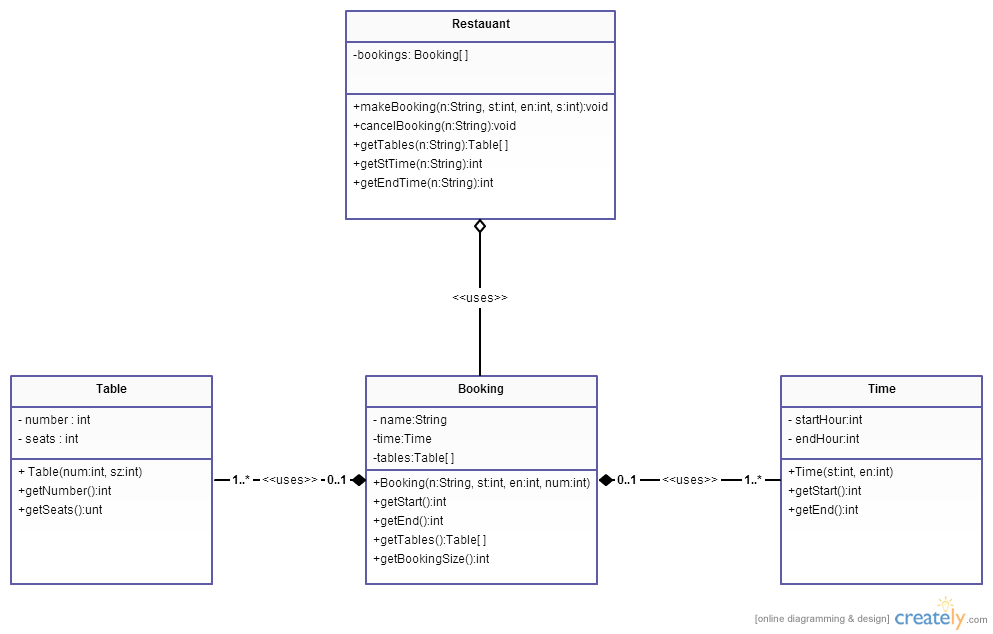
\includegraphics[width=1\textwidth]{restarentbooking.png}\\
	\figcaption{Restaurant Reservation System}\label{fig:rbooking}
\end{center}

\section{Poker Game}
Implement Poker game

\section{Three Stacks}
 Implement three stacks using single array.
 
 \section{C++Garbage}
 Design garbage collector of C++
 
 \section{Alarm Clock}
 design an alarm clock for a deaf person.
 
 \begin{Code}
 	//Vibrator, light \& pillow vibrator. To cover minimal to severely deaf. 
 	//Vibrator + Light = Normal deaf. 
 	//Pillow vibrator + Light = severely deaf.
 	Class Clock
	 	Set the time.
	 	Advance the time.
	 	Display the time.
 	
 	Class Hour indicator
	 	Set its value
	 	Advance its value
	 	Display its value
 	
 	Class Minute indicator
	 	Set its value
	 	Advance its value
	 	Display its value
 	
 	Class Seconds indicator
	 	Advance its value
	 	Display its value
 	
 	Vibrator
	 	Trigger
	 	Silent
 	
 	Light
	 	On
	 	Off
 \end{Code}